\subsection{单例模式(Singleton)}

\subsubsection{单例模式简介}

单例模式是一种常用的软件设计模式,它保证一个类只有一个实例,并提供一个全局访问点来访问该实例。

单例模式通常用于某个类需要在整个应用程序中只有一个实例的场景,例如系统的配置类或者线程池。

要实现单例模式,一般需要将类的构造函数设为私有的,并且提供一个静态方法用于获取该类的唯一实例。这样,在整个应用程序中就只能通过这个静态方法来访问该类的实例。

单例模式有一些优点:

可以保证一个类只有一个实例,避免了对象的多次创建,降低了系统的内存开销。

可以提供一个全局访问点,方便访问该实例,避免了创建多个实例带来的麻烦。

可以提供一个统一的访问接口,方便维护和扩展该实例。

但是,单例模式也有一些缺点:

单例类的扩展有一定的困难,因为单例类的实例数量是固定的。

如果单例类中存在大量长生命周期的资源,那么单例模式还有一个缺点就是难以测试,因为它的实例是全局的,如果要测试单例类的方法,那么需要改变全局的实例,这样就会影响到其他的测试用例。

在实际开发中,需要根据实际情况来判断是否使用单例模式。如果需要保证一个类只有一个实例,并提供一个全局访问点,那么可以考虑使用单例模式。

\subsubsection{单例模式在项目中的应用}

\begin{figure}[htb]
  \centering
  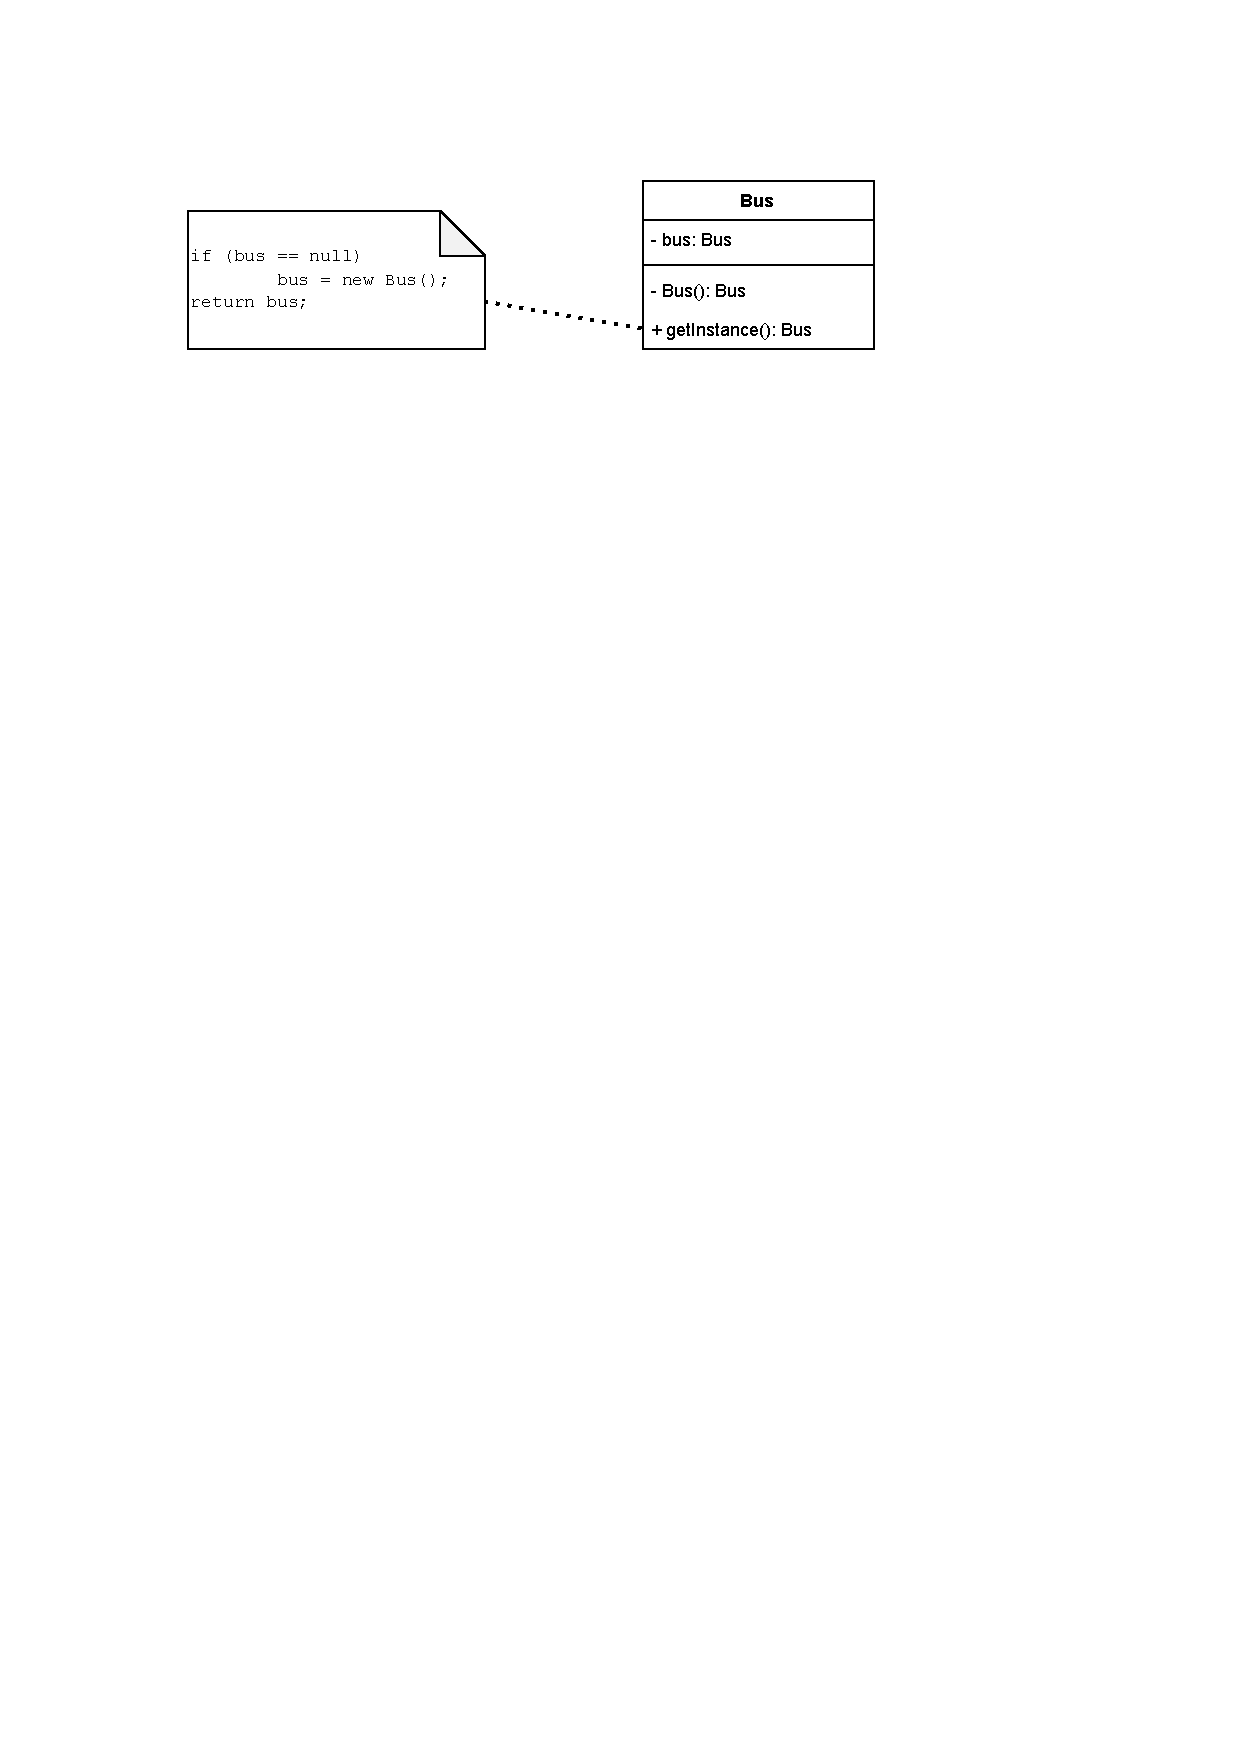
\includegraphics[width=0.9\textwidth]{figures/单例.pdf}
  \caption{单例模式在 Slow6502 中的类图}
\end{figure}

本项目中CPU的Bus类被设计为单例模式,因为我们的CPU的Bus始终只能有一个。这样设计可以确保一个项目中只存在一个 Bus 对象,这样可以避免在项目中出现多个不同的 Bus 对象造成的冲突。另外,使用单例模式还可以提高系统的效率,因为在整个程序运行期间,它只会创建一个 Bus 对象,而不会每次都创建一个新的对象。

此外,通过将 Bus 类设计为单例模式,可以更容易地访问和控制 Bus 类的实例。例如,在项目中可以通过调用单例类的静态方法来访问 Bus 对象,这样就可以确保所有对 Bus 类的访问都是通过同一个对象进行的。这有助于提高系统的一致性和可靠性。

